%%% Um einen Artikel auf deutsch zu schreiben, genügt es die Klasse ohne
%%% Parameter zu laden.
\documentclass[biblatex]{lni}
\addbibresource{bibliographie.bib}
%%% To write an article in English, please use the option ``english'' in order
%%% to get the correct hyphenation patterns and terms.
%%% \documentclass[english]{class}
%%
\usepackage[caption=false]{subfig}
\usepackage{acronym}
\usepackage{float}
\usepackage{tikz}
\begin{document}
%%% Mehrere Autoren werden durch \and voneinander getrennt.
%%% Die Fußnote enthält die Adresse sowie eine E-Mail-Adresse.
%%% Das optionale Argument (sofern angegeben) wird für die Kopfzeile verwendet.
\title[Auswirkungen von SOA]{Auswirkungen einer serviceorientierten Architektur auf den Entwicklungs- und Auslieferungsprozess}
%%%\subtitle{Untertitel / Subtitle} % if needed
\author[Fabian Klimpel \and Lukas Epple \and Raphael Sack]
{Fabian Klimpel\footnote{DHBW Stuttgart Campus Horb, Florianstraße 15, 72160 Horb, Deutschland \email{i20021@hb.dhbw-stuttgart.de}} \and
Lukas Epple\footnote{DHBW Stuttgart Campus Horb, Florianstraße 15, 72160 Horb, Deutschland \email{i20009@hb.dhbw-stuttgart.de}} \and 
Raphael Sack\footnote{DHBW Stuttgart Campus Horb, Florianstraße 15, 72160 Horb, Deutschland \email{i20029@hb.dhbw-stuttgart.de}}}
\editor{Prof. Dr.-Phil. Antonius van Hoof} % Names of Editors
\booktitle{Advanced Software-Engineering} % Name of book title
\yearofpublication{2022}
%%%\lnidoi{18.18420/provided-by-editor-02} % if known
\maketitle

\begin{abstract}
    Das Konzept der serviceorientierten Architektur (SOA) existiert schon seit den 1990er Jahren und wird zunehmend in größeren Softwaresystemen eingesetzt. Während diese Architektur viele Vorteile mit sich bringt, bietet die Umsetzung dieser auch viele Herausforderungen. Ziel dieser Arbeit ist es die Vor- und Nachteile der serviceorientierte Architektur zu dokumentieren und Unterschiede zu anderen konventionellen Software-Architekturen, insbesondere hinsichtlich der Entwicklung und Auslieferung aufzuzeigen.  Dabei soll vor allem der Kontext der agilen Softwareentwicklung betrachtet werden. Für einen qualitativen Vergleich wurde eine umfassende Literaturrecherche durchgeführt. Die Recherchen zeigten, dass insbesondere die Qualität von umfangreichen und komplexen Softwaresysteme vom Einsatz der serviceorientierten Architektur und deren Auswirkungen auf den Entwicklungs- und Auslieferungsprozess profitieren kann.
\end{abstract}
\begin{keywords}
SOA \and serviceorientierte Architektur \and Software-Engineering \and Software Architektur%Keyword1 \and K   eyword2
\end{keywords}
%%% Beginn des Artikeltexts
\section{Einleitung}
\section{Geschichtliche Entwicklung}
\label{ch:history}

Um die Notwendigkeit der serviceorientierten Architektur nachvollziehen zu können, lohnt es sich die Vergangenheit - vor SOA - anzusehen. In diesem Kapitel wird die Entwicklung von Software-Architekturen vom Monolithen bis hin zur Serviceorientiertheit betrachtet.

\subsection{Monolithische Architektur}
\label{sec:monolithicArch}

Als monolithisch werden Objekte bezeichnet, die \glqq aus einem Stück bestehen[.]; zusammenhängend und fugenlos [sind]\grqq{} \cite{Duden.monolithisch.25.10.2022}. Im Kontext des Software-Engineerings sind damit jegliche Anwendungen gemeint, deren Module nicht unabhängig voneinander ausgeführt werden können und deren Funktionalitäten in einer Applikation gekapselt sind \cite{Ponce.2019}.

Während den Anfängen des Software-Engineerings und bevor das Fachgebiet der Software-Architektur existiert hatte, existierten fast ausschließlich Monolithen \cite{Kruchten.2006}.  

Ende der 1960er Jahre gab es die ersten Bemerkungen, Software nicht nur als \glqq amorphous lump of program\grqq{} \cite{Kruchten.2006}[S.24] anzusehen, sondern gezielt die Architektur eines Software-Systems zu designen.

Monolithen haben noch heute ihre Daseinsberechtigung. Gerade kleine stand-alone Anwendungen werden häufig von einem Service dargestellt. Der große Vorteil dabei ist das einfache Testen \cite{Ponce.2019}. Einzelne Dienste einer Anwendung müssen nicht mit Integrationstests auf verschiedenen Status abgebildet werden, da es nur einen Dienst zum Testen gibt. Auch das Deployment ist simpel, da es nur aus einer ausführbaren Komponente besteht. 

Durch die \glqq fehlende\grqq{} Architektur wird zunächst Zeit gewonnen, da weniger geplant werden muss. Für kleine Projekte oder Prototypen ist das ideal. Gerade bei Letzterem können durch den erstmaligen Aufbau im Monolith die Komplexität und einzelne Komponenten erforscht werden \cite{Ponce.2019}. Aber bei großen Projekten geht schnell der Überblick verloren und die Entwicklung kommt ins Stocken \cite{Ponce.2019}. 

Die Entwicklung einer monolithischen Anwendung bedeutet eine enge Bindung zur genutzten Technologie \cite{Ponce.2019}. Falls der Support verwendeter Drittanbieter-Software ausläuft, oder neue Schwachstellen gefunden werden, ist es nur schwer möglich Änderungen vorzunehmen. Und gleichzeitig: Egal wie groß oder klein eine Anpassung ist, die gesamte Anwendung muss immer neu getestet, gebaut und verteilt werden. Falls ein Laufzeitfehler auftritt, hat dies den Absturz der gesamten Anwendung zur Folge \cite{Ponce.2019}. Und obwohl solch ein Bug durch eine kleine Modifikation gefixt werden kann. Manchmal ist ein neuer Build zu aufwändig und es wird auf mehrere Änderungen gewartet. Darunter leidet die Qualität der Software. Auch lässt sich die Applikation nicht beliebig skalieren. Durch zum Beispiel Load Balancer kann die gesamte Anwendung horizontal skalieren, nicht jedoch einzelne Komponenten.

Zusammenfassend: Monolithen sind gut für kleine Projekte, oder erste Proof of Concepts. Falls eine Software jedoch nachhaltig, mehrere Jahre lang zuverlässig betreut und weiterentwickelt werden soll, steigt die Komplexität dieser drastisch mit der Zeit. Neue Teammitglieder müssen sich teilweise in die komplette Codebase einarbeiten, um Änderungen vorzunehmen. Es kann auch dazu kommen, dass keine neuen Arbeitskräfte gefunden werden die sich mit 20 Jahre alter Software-Technologie auseinandersetzen wollen und somit ist eine Neuentwicklung früher oder später unumgehbar. 

Wenn Architekturen - und damit der Aufbau von Software - verglichen werden, dann wird dies mithilfe von \glqq fundamentalen Grundprinzipien\grqq{} getan \cite{FrankBuschmann.}. Im Folgenden werden diese Punkte aufgezählt um zu zeigen, gegen welche Grundprinzipien die monolithische Architektur verstößt. In den darauf folgenden Kapiteln werden Architekturen gezeigt die iterativ verschiedene Probleme lösen, welche letztendlich einen historischen Verlauf zu SOA aufzeigen soll:
\begin{itemize}
    \item \textbf{Abstraktion}: \glqq Die essenziellen Eigenschaften eines Objekts, die es von allen anderen Arten von Objekten unterscheidet und somit klar definierte konzeptionelle Grenzen in Bezug auf die Perspektive des Betrachters setzt\grqq{} \cite{Booch.1993}. In einem Monolith kann es keine echte Abstraktion geben, da die Software nur aus einem Objekt - sich selbst - besteht. Natürlich existieren auf einem niedrigeren Level eine Abstraktion, aber nicht in der Architektur selbst.
    \item \textbf{Kapselung}: Durch die Verkapselung verschiedenster Abstraktionen können diese gruppiert und auseinander gehalten werden. Dies fördert die Änderbarkeit und Wiederverwendbarkeit \cite{FrankBuschmann.}. Die Kapselung, zum Beispiel von Klassen einer Programmiersprache kann auch für Monolithen existieren, aber nicht in einer Form, die eine Wiederverwendbarkeit anstrebt.
    \item \textbf{Modularisierung}: Hierbei geht es um die sinnvolle Zerlegung eines Softwaresystems und dessen Gruppierung in Subsysteme und Komponenten. Module dienen als physische Container für Funktionalitäten oder Verantwortlichkeiten einer Anwendung. \cite{FrankBuschmann.}. Wie bei vielen dieser Prinzipien lässt die monolithische Architektur Modularisierung zu einem gewissen Grad zu, aber nur auf einem niedrigen Level.
    \item \textbf{Trennung von Verantwortlichkeiten}: Unterschiedliche Verantwortlichkeiten innerhalb eines Softwaresystems sollten voneinander getrennt werden. 
    \item \textbf{Kopplung und Kohäsion}: Die Kopplung ist das Maß für die Stärke der Assoziation zwischen Modulen. Eine Starke Kopplung verkompliziert das System \cite{FrankBuschmann.}. Kohäsion misst den Grad der Konnektivität zwischen den Funktionen und Elementen eines einzelnen Moduls.
    \item \textbf{Suffizienz, Vollständigkeit und Primitivität}: Suffizienz meint, dass eine Komponente alle notwendigen Merkmale einer Abstraktion erfasst und eine sinnvolle und effiziente Interaktion ermöglicht. Vollständigkeit heißt, dass alle relevanten Merkmale erfasst werden. Mit Primitivität ist gemeint, dass jede Operation, die eine Komponente ausführen kann, einfach implementiert werden kann \cite{FrankBuschmann.}.
    \item \textbf{Single Point of Reference}: Jede Entität innerhalb eines Softwaresystems sollte nur einmal definiert werden. Dadurch entstehen keine inkonsistenten Zustände.
\end{itemize}

\subsection{Schichtenarchitektur}
\label{sec:layeredArch}

Die Schichtenarchitektur war eines der ersten Architektur-Pattern mit welchem versucht wurde die Probleme einer monolithischen Architektur zu lösen \cite{SavolainenJuha.2009} und ist bis heute wahrscheinlich einer der am häufigsten angewendeten Software-Architekturen (vor allem im Web).

Ein Programm wird dabei in $n$ Schichten aufgeteilt, jede Schicht ist ein Modul der Software und kommuniziert über Protokolle mit anderen Schichten. Die Aufteilung alleine löst schon fast alle oben genannten Probleme. Die Schichten bilden meist eine Hierarchie ab, wobei die Kommunikation nur strikt durch gewisse Schichten geschieht. 

Vor allem lassen sich Verantwortlichkeiten sehr gut damit trennen. Als Beispiel, kann das 3-Schichten Modell aus typischen Web-Anwendungen betrachtet werden\footnote{Auch wenn dies ein prominentes Beispiel ist, besteht eine Schichtenarchitektur nicht immer aus 3 Schichten}:
\begin{enumerate}
    \item \textbf{Präsentationsschicht}: das Frontend als grafische Benutzeroberfläche im Browser.
    \item \textbf{Anwendungsschicht}: die eigentliche Funktionalität der Software abgeschottet von Anwendenden.
    \item \textbf{Datenschicht}: eine Datenbank, auf der die Anwendungsdaten verwaltet werden.
\end{enumerate}

Bei der Modellierung können die Schichten einzeln betrachtet werden, um Schnittstellen zu definieren. Entwicklerteams können daraufhin gleichzeitig an Front- und Backend arbeiten und sind dabei technologisch unabhängig voneinander. Und im Laufe des Lebenszyklus der Anwendung können einzelne Schichten ausgetauscht werden, um neue Technologie einzusetzen. Weitere Vorteile sind auch, dass sich die Geschäftslogik direkt im Code befindet und dass geheime Informationen nicht öffentlich für Benutzer zugänglich sind, sondern sich auf einer unzugänglichen Schicht befinden.

Für große Projekte mit größeren Teams ist es leichter Software in Schichten zu schreiben. Einzelne Teams können sich dabei auf eine bestimmte Schicht spezialisieren, um effizienter zu sein. 

Die Verteilung von Software bringt auch Nachteile mit sich, bzw. alle Vorteile der monolithischen sind die Nachteile von dieser Architektur:
\begin{itemize}
    \item Das Testen ist wesentlich aufwändiger. Unit-Tests sind auf den einzelnen Schichten unverändert, aber bei der Integration aller Schichten ist es schwer alle Testfälle abzudecken bzw. die Tests überhaupt zu schreiben.
    \item Die Installation von Software ist wesentlich aufwändiger, da mehrere Schichten meist über das Internet kommunizieren müssen.
    \item Der Planungsaufwand ist höher und vor allem kleine Projekte könnten unnötig Zeit an der Trennung der Schichten verlieren. Macht sich aber in der späteren Betreuung des Codes bezahlt.
\end{itemize}

Zusammengefasst lässt sich sagen: Die Schichtenarchitektur teilt \textbf{eine} Software in \textbf{verschiedene} Schichten auf. Dabei muss stets auf die Balance zwischen Kopplung und Kohäsion geachtet werden. Die Schichten können dabei verschiedenste Technologien implementieren, solange diese mithilfe wohl definierter Protokolle kommunizieren können. Die Schichten können in der Entwicklung anderer Software wiederverwendet werden, was die Entwicklung in Zukunft erleichtert. Aber die Architektur zeigt ebenfalls Probleme auf. Die Schichten trennen zwar zu einem gewissen Grad die Verantwortlichkeiten der Software, aber für große Projekte ist die statische Hierarchie der Schichten nicht fördernd. Oftmals werden bei einer 3-Schichten Architektur auch nur 2 große Monolithen entwickelt (mit einer Datenschicht) \cite{FrankBuschmann.}. 

\subsection{Serviceorientierte Architektur}
\label{sec:historySoa}

Die Herausforderung der Schichtenarchitektur kann gelöst werden, indem die \glqq Schichten\grqq{} granularer werden. Und anstatt diese in einer festen Hierarchie anzuordnen - wo zum Beispiel Schicht $n$ nur mit Schicht $n+1$ kommuniziert - gibt es eine liberalere Kommunikation, die nicht mehr statisch vorgegeben sein muss. Anstatt, dass eine Schicht für die gesamte Geschäftslogik einer Anwendung zuständig ist, werden weitere Verantwortlichkeiten innerhalb dieser in Services aufgeteilt. Dadurch wird eine losere Kopplung und eine erhöhte Kohäsion erreicht. 

Dieses Ziel hat gerade für große Softwareunternehmen einen immensen Vorteil. Anstatt einzelne Services nur in der Entwicklung wiederzuverwenden, können diese jetzt zur Laufzeit wiederverwendet werden. Die Verantwortlichkeiten sind so granular, dass sich diese in anderen Projekten unverändert wiederverwenden kann.

Langfristig bilden sich nur geringe Kosten durch den hohen Grad der Wiederverwendbarkeit der Dienste, aber bei diesem Grad der Granularität stößt die serviceorientierte Architektur an einen großen Overhead der auch Probleme mit sich bringt \cite{SolutionsMartinSchmidtAsgard.26.11.2022}:\begin{itemize}
    \item Die Analyse, Konzeption und Implementierung ist initial wesentlich höher als bei anderen Architekturen.
    \item Die Wiederverwendbarkeit kann auch ein Problem darstellen, da dies nur eingeschränkt und nur auf sehr langer Zeit gesehen möglich ist. Das erfordert eine noch genauere Planung für die Zukunft.
    \item Die Granularität erhöht die Anzahl der Schnittstellen, deren Änderungen oftmals zu Kompatibilitätsproblemen führen können (=erhöhte Komplexität).
    \item In der Regeln hat eine SOA-Anwendung eine schlechtere Performance und höheres Datenvolumen, da die Dienstkommunikation höhere Latenzen darstellt.
    \item Die Bereitstellung und Konfiguration der Bindung zwischen den Diensten ist häufig komplex und Themen wie die Authentifizierung/Autorisierung sind Herausforderungen die mit hohen Kosten verbunden sind.
    \item Entwicklerteams müssen über ein breiteres Wissen verfügen um SOA wirklich anwenden zu können.
    \item Die Kostenverwaltung der Entwicklung einer zentralen und Abteilungsübergreifenden SOA ist eine politische Herausforderung und muss von Mitarbeitenden unterstützt werden.
\end{itemize}

Die Information, die aus diesem Kapitel herausstechen sollte, ist die Tatsache, dass sich SOA erst bezahlbar macht, nachdem die gesamte Architektur steht. Bis zu diesem Punkt sind immense Aufwände seitens des Unternehmens notwendig. Bei kleinen bzw. neuen Softwareunternehmen ist der Systemaufbau mit SOA meist zu teuer und würde sich nicht lohnen, bzw. bei einer Gründung ist es schwer in die Zukunft zu blicken, um die richtigen Services herauszusuchen. Für bestehende Unternehmen heißt eine SOA, die Neuentwicklung der Softwarelandschaft. Ein Transformationsprojekt hin zu SOA kann Jahre dauern und ist ein großes  für die Zukunft. Die abgeschlossene Transformation macht sich jedoch bezahlt. 

Interessant zu sehen: bei diesen Architekturen gibt es einen Trade-off zwischen Komplexität in der Planung und der Komplexität in der Pflege/Entwicklung. Die Gesamtkosten eines Projektes sollten unabhängig von der Wahl einer Architektur sein, jedoch werden die Kosten und Aufwände anders über den Projektlebenszyklus verteilt. 

\newpage
Monolithen haben wenig initiale Aufwände, aber die spätere Pflege ist mit einem hohen Kostenaufwand verbunden. SOA hat immense Anfangskosten, welche nach dem Aufbau der Architektur wieder fallen. Und die Schichtenarchitektur ist eine Balance dazwischen. Monolithische Projekte können ohne viel Aufwand angefangen werden und falls diese ohne Abschluss scheitern, so wurde nur der minimale Aufwand erreicht. Im Gegensatz dazu kostet ein gescheitertes SOA-Projekt wesentlich mehr Geld und Aufwände, da das meiste davon in der Planung (am Anfang) aufgebracht wird.

\begin{figure}[H]
    \centering
    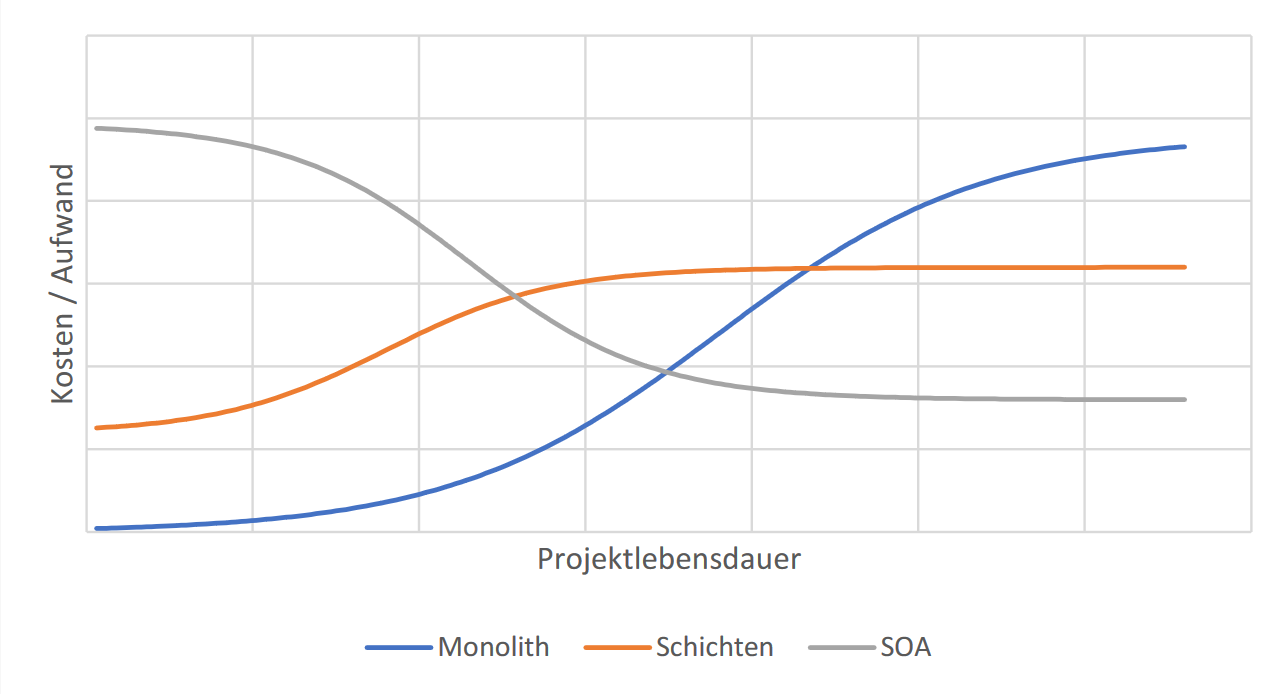
\includegraphics[width=.9\textwidth]{images/archgraph.png}
    \caption{Relativer Kosten-/Aufwand-Vergleich der vorgestellten Architekturen}
\end{figure}

Trotzdem kann sich der Umstieg zu einer serviceorientierten Architektur lohnen. Im Nachfolgendem wird tiefer darauf eingegangen wie sich SOA auf den Entwicklungs- und Auslieferungsprozess in der agilen Softwareentwicklung auswirkt.

\section{Realisierung einer SOA}
\label{ch:realization}

% Aufteilung in Services

Es gibt viele unterschiedliche Wege eine SOA in der Praxis zu realisieren. Eine der verbreitetsten Möglichkeiten eine serviceorientierte Architektur zu realisieren ist mit Web-Services. Weitere Technologien zur Implementierung von SOA ist der Komponentendienst COM+ von Microsoft, Java 2 Platform Enterprise Edition (J2EE) oder die CORBA-Spezifikation. Im Folgenden werden jedoch nur Web-Services betrachtet, da dies der verbreitetste Weg ist eine SOA zu implementieren.


\begin{figure}[H]
    \centering
    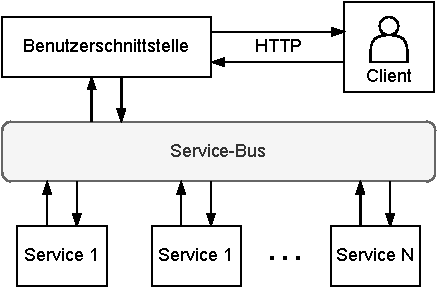
\includegraphics[width=.7\textwidth]{images/SOA-Service-Bus.drawio.pdf}
    \caption{SOA Aufbau}
    \label{fig:soa-aufbau}
\end{figure}

Wichtig zu sagen ist noch, dass es nicht nur einen richtigen Weg gibt, eine SOA zu implementieren. Es gibt meist viele verschiedene Wege, welche zum gewünschten Ziel führen können. In der Regel müssen mehrere Services implementiert werden, welche gemeinsam über einen Service-Bus miteinander kommunizieren können. Je nach expliziter Implementierung ist der Service-Bus dabei eine globale Instanz über die gesamte Applikation hinweg, oder eine Abstraktion für direkte Verbindungen zwischen verschiedenen Services. In Abbildung \ref{fig:soa-aufbau} wird ein beispielhafter Aufbau einer serviceorientierten Architektur dargestellt. Der Service-Bus ist dabei eine Abstraktion der Schnittstellen und an ihn angebunden sind verschiedene Service-Komponenten. Einer der Services ist dabei die Benutzerschnittstelle, mit der die Benutzer zum Beispiel über ein Frontend interagieren können.

\textbf{Service-Bus}

Mit der wichtigste Bestandteil eines Services ist seine Schnittstelle. Für die Realisierung der Schnittstelle kommen zwei verschiedene Designprinzipen infrage. Entweder ein nachrichtenorientiertes Design oder ein hypermedia-gesteuertes Design.\\
Bei dem nachrichtenorientierten Design kommunizieren die Services über einen Service-Bus. Über diesen können die einzelnen Komponenten Nachrichten austauschen. In der Regel wird dabei ein Message-Broker oder eine direkte Kommunikation der Services über TCP/IP verwendet. Für die Kommunikation zum Konsumenten wird in der Regel eine HTTP-API bereitgestellt.\\
Die zweite Möglichkeit ist die hypermedia-gesteuerte Implementierung. Im Gegensatz zur nachrichtenorientierten Implementierung werden bei der hypermedia-gesteuerten Implementierung nicht nur Daten, sondern auch Inhalte mit Beschreibungen möglicher Aktionen ausgetauscht. Dabei wird zum Beispiel direkt HTML Quelltext mit einer Form zurückgegeben. Dies ist vorteilhaft, wenn der Konsument über eine Webseite auf einen Service zugreifen will. \cite{NADAREISHVILI.2016}

Für die eigentliche Implementierung von dem Service-Bus gibt es viele Möglichkeiten. Ein Service-Bus kann beispielsweise als separate Software-Komponente implementiert werden. Der Service-Bus kann dabei von Grund auf implementiert werden oder es kann ein bestehender Message-Broker wie zum Beispiel RabbitMQ verwendet werden. Dabei kann der Service-Bus Nachrichten empfangen und über Routing an den richtigen Service weiterleiten. Der Vorteil daran ist, dass der Service-Bus dabei beliebig skaliert werden kann. Eine weitere Möglichkeit wäre eine in die Services integrierte Middleware, welche die benötigten Schnittstellen zur Kommunikation unter den Services zur Verfügung stellt. Dabei werden üblicherweise Web-Protokolle wie SOAP oder REST eingesetzt. \cite{Heutschi.2007}

% Service Provicer - Service Customer

% Service Bus
%   - Message Broker
%   - (REST) APIs
%   - IPC

% API Design:
%   - Nachrichtenorientiert
%   - Hypermedia-Driven
% https://docs.broadcom.com/doc/microservice-architecture-aligning-principles-practices-and-culture S. 67

% \subsection{Modellierung}

% Schnittstellenbasierte oder Komponentenbasierte Modellierung bietet sich an. Dafür bietet sich UML ab der Version 2.0 an, da dort wesentliche Verbesserungen in der Darstellung von Komponenten und Kontroll- und Ablaufkonzepte beinhaltet. 

% A Service Component is an encapsulated, autonomous software entitiy that realizes and provides the Service through its interface in a contract-based fashion without exposing its internal implementation

\textbf{Service-Komponente}

% Jede Service-Komponente erfüllt eine kleine Funktionalität der Applikation

Eine Service-Komponente ist eine Software-Entität, welche als eigenständige, unabhängige und in sich geschlossene Einheit mit einem klaren Zweck besteht. Die Komponente ist dabei eine unabhängige Einheit von einer Funktionalität mit standardisierten Schnittstellen zur Kommunikation mit anderen Komponenten in einer Anwendung. In der Regel hat die Service-Komponente eine eindeutige Funktion, welche unabhängig von anderen Service-Komponenten der Anwendung ist.

Die eigentliche Implementierung des Services kann in einer beliebigen Programmiersprache geschehen. Es können auch unterschiedliche Services in unterschiedlichen Programmiersprachen implementiert werden. Dabei kann individuell für die Funktionalität eines jeweiligen Services eine optimale Programmiersprache verwendet werden. Wichtig ist dabei lediglich, dass die Schnittstellen korrekt angesprochen werden.   

% Die Basiselemente einer Service-Komponente sind sein Kontext, Kontrakt und Realisierung. Die Rolle eines Services ist in seinem Kontrakt spezifiziert. Der Kontrakt wird durch die Realisierung der Service-Komponente realisiert, die durch eine Schnittstelle vor dem Kontext verborgen ist. Mehrere Service-Komponenten, welche im selben Kontext zusammenarbeiten, werden als Choreografie bezeichnet. In Abbildung \ref{fig:component-metamodell} ist das Service-Komponenten-Metamodell dargestellt. \cite{Stojanovic.op.2004}

% \begin{figure}[H]
%     \centering
%     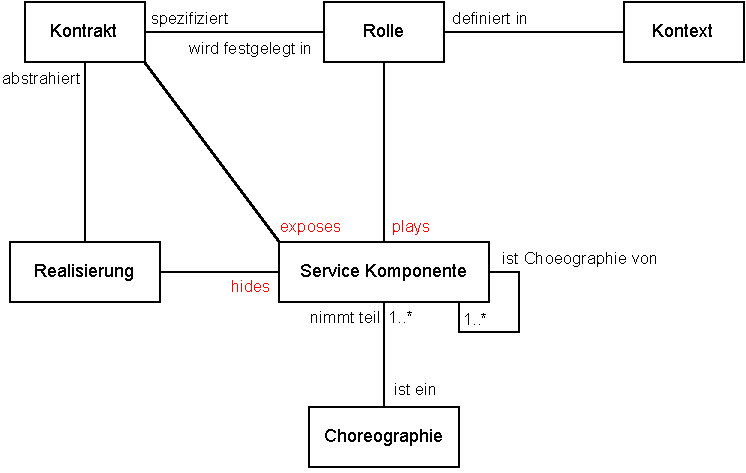
\includegraphics[width=1.\textwidth]{images/Service-Komponent-Metamodell.drawio.pdf}
%     \caption{Service-Komponenten-Metamodell}
%     \label{fig:component-metamodell}
% \end{figure}

\begin{figure}[H]
    \centering
    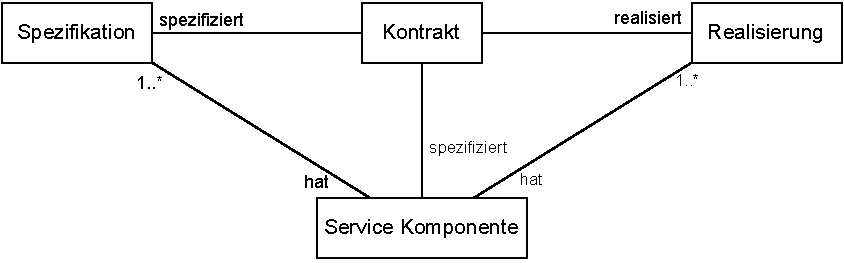
\includegraphics[width=1.\textwidth]{images/Spezifikation-Realisation-Service.drawio.pdf}
    \caption{Spezifikation und Realisation einer Service-Komponente \cite{Stojanovic.op.2004}}
    \label{fig:specification-realisation}
\end{figure}

Die Basiselemente für die Planung und Umsetzung einer Service-Komponente sind die Spezifikation, der Kontrakt und die Realisierung. Die Zusammenhänge der Basiselemente sind in Abbildung \ref{fig:specification-realisation} dargestellt. Im Kontrakt sind dabei die Regeln und Anforderungen der Service-Komponente spezifiziert. Also der Funktionsumfang, welcher der Service bereitstellen soll. Dieser Kontrakt wird in der Spezifikation weiter spezifiziert. In der Spezifikation wird die Art und die Verwendung der Schnittstellen definiert. Darunter zählen zum Beispiel die verwendeten Protokolle und Standards für die Kommunikation und die Information welche Funktionen von dem Service bereitgestellt werden. Wurde alles korrekt spezifiziert kann der Service-Kontrakt implementiert werden. Für die Benutzung des Services ist dessen Implementierung nicht von Bedeutung, solange der Kontrakt des Services voll erfüllt wurde. \cite{Stojanovic.op.2004}

\subsection{Konzepte und Technologien}
\label{sec:conceptsAndTechnologies}

In der serviceorientierten Architektur gibt es keine Vorschriften wie genau etwas zu implementieren ist und welche Technologie dabei verwendet werden soll. Jedoch gibt es einige Technologien und Konzepte, welche sich in dem Bereich der SOA etabliert haben. Die Wahl der explizit zu verwendeten Technologien ist dabei von den Anforderungen der Anwendung abhängig. Bei der Planung und dem Design sollten die Technologien jedoch genau spezifiziert werden, welche anschließend zur Implementierung verwendet werden.

Die verbreitetste Technologie zur Umsetzung von SOA sind Web-Services. Web-Services kommunizieren über standardisierte Schnittstellen in einem Netzwerk miteinander. Dabei funktioniert die Kommunikation über Netzwerkprotokolle wie zum Beispiel SOAP oder REST. \cite{Heutschi.2007}

\begin{figure}[H]
    \centering
    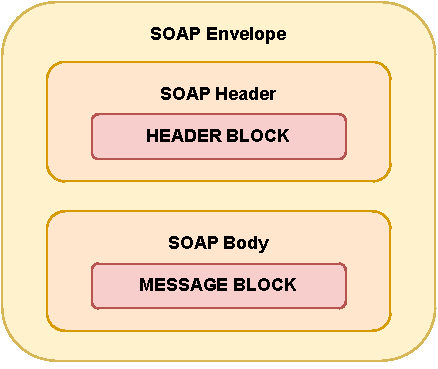
\includegraphics[width=.5\textwidth]{images/SOAP.drawio.pdf}
    \caption{SOAP Aufbau \cite{AlexanderS.Gillis.02.12.2022}}
    \label{fig:soap}
\end{figure}


Das Simple Object Access Protocol (SOAP) benutzt in der Regel das HTTP-Protokoll zur Datenübertragung. Dabei werden die Daten in Form von XML gesendet. SOAP ist unabhängig von der verwendeten Programmiersprache und wird meist in verteilten Systemen und somit auch in SOA verwendet. Der Aufbau einer SOAP-Komponente ist in Abbildung \ref{fig:soap} dargestellt. Außen befindet sich der SOAP Envelope, welcher alle Daten enthält und das XML-Dokument als SOAP-Nachricht identifiziert. In dem SOAP Envelope befindet sich ein Header und ein Body. Der Header beinhaltet dabei zusätzliche Informationen über die Nachricht. Dies sind zum Beispiel zusätzliche Daten zur Authentifizierung. Im Body steht der eigentliche Inhalt der Nachricht. SOAP kann sowohl für Anfragen an einen Service, als auch für dessen Antwort verwendet werden. \cite{AlexanderS.Gillis.02.12.2022}

Der Aufbau in Abbildung \ref{fig:soap} wird wie folgt im XML-Format geschrieben: 

\begin{lstlisting}
<?xml version="1.0"?>
<soap:Envelope xmlns:soap="http://www.w3.org/2003/05/soap-envelope/">
    <soap:Header>
        HEADER BLOCK
    </soap:Header>
    <soap:Body>
        MESSAGE BLOCK
    </soap:Body>
</soap:Envelope>
\end{lstlisting}

Um einen Service und vor allem dessen Schnittstellen zu beschreiben kann die Web Services Description Language (WSDL) verwendet werden.\\
WSDL ist ein Standardformat um einen Web-Service zu beschreiben. Die Beschreibung des Services wird in dem XML-Format in der WSDL-Datei definiert. Neben einer Beschreibung der Funktionalität des Services sind auch alle Informationen, um mit einem dem Web-Service zu kommunizieren, darin enthalten. \cite{Heutschi.2007}

Häufig wird WSDL in Verbindung mit SOAP verwendet. Dabei kann der Client, welcher den Service anfragt, die WSDL Datei einlesen, um somit die verfügbaren Funktionen des Services abzurufen. Nun kann er die in WSDL definierten verfügbaren Funktionen über das SOAP-Protokoll verwenden. \cite{Heutschi.2007}

Für die Umgebung, in der die Services ausgeführt werden, bietet sich eine skalierbare Cloud-Infrastruktur an, bei der eine schnelle Bereitstellung an Rechenkapazitäten und ein automatisches Deployment der Services realisiert werden kann. 

% WSDL:
% - Standardformat um einene Web-Service zu beschreiben
% - XML-Datei
% - beinhaltet alle Informationen um mit einem Web-Service zu kommunizieren  (Interface)
% - Beschreibt die Funktionalität eines Web-Services

% Web Services: WSDL, SOAP
% Messaging: RabbitMQ
% REST
% OPC-UA

% - Programmiersprache, welche web API freundlich ist
% - Programmiersprache, welche den Kompetenzen des Entwicklerteams entspricht

\subsection{Sicherheitskritische Aspekte der SOA}
\label{sec:securityAspects}

Eine serviceorientierte Architektur ist ohne IT-Sicherheit nicht denkbar. Neben klassischen, bei jeder IT-Lösung, auftretenden Aufgaben gibt es auch - durch den verteilten Ansatz von SOA - spezielle Anforderungen an das System \cite{BITKOM.2009}.

Die einzelnen Aufgaben müssen dabei nicht neu erfunden werden, sondern haben lediglich besondere Ausprägungen in der Anwendung von SOA. In allen Fällen muss sich mit folgenden Problemen befasst werden \cite{BITKOM.2009}:\begin{itemize}
    \item Identitätsverwaltung
    \item Authentisierung
    \item Autorisierung (=Access Control)
    \item und die verschlüsselte Kommunikation zwischen den Diensten.
\end{itemize}

Nachfolgend wird beschrieben, wieso diese Aufgaben gerade in SOA kritische Herausforderungen sind und wie sie gelöst werden.

\paragraph{Access Control:}

In einer SOA müssen nicht nur viele Benutzer, sondern auch Dienste authentifiziert werden. Die Verwaltung dieser Identitäten, insbesondere über Organisationsgrenzen hinweg ist eine Notwendigkeit \cite{BITKOM.2009}.

Bei SOA existieren - anders als bei monolithischen Architekturen - viele potenzielle Schwachstellen an jedem Service. Wird eine davon ausgenutzt, so ist zwar nur ein kleiner Teil der Anwendung kompromittiert, aber die Sicherheit des Gesamten ist nicht mehr vorhanden.

Jeder einzelne Service sollte ausreichend mit geschützt sein, damit nur autorisierte Identitäten Zugriff auf eine Ressource haben. Gleichzeitig sollten Benutzer sich nicht bei jedem Service einzeln anmelden, da es nicht benutzerfreundlich ist.

Dies kann erreicht werden, indem bestehende Sicherheits-Architekturen oder Standards in SOA als weitere Services integriert werden. Der Hauptzweck hinter all diesen Standards ist die Orchestrierung der Authentifizierung zwischen mehreren Diensten.

Die dabei am häufigsten verwendeten Standards sind:\begin{itemize}
    \item \textbf{XACML}: Dieser Standard besteht aus mehreren Services (Points), welche anhand von Policies Anfragen einer Entität bewerten und gegebenenfalls weiterleiten. \glqq XACML bleibt die einzige standardisierte Methode zur dynamischen Durchsetzung von Autorisierungen, indem Zugriffskontrollen von Anwendungen und Datenbanken ausgelagert und Geschäftsrichtlinien verwendet werden.\grqq{} \cite{Axiomatics.03.08.2022}\\
    \begin{figure}[H]
        \centering
        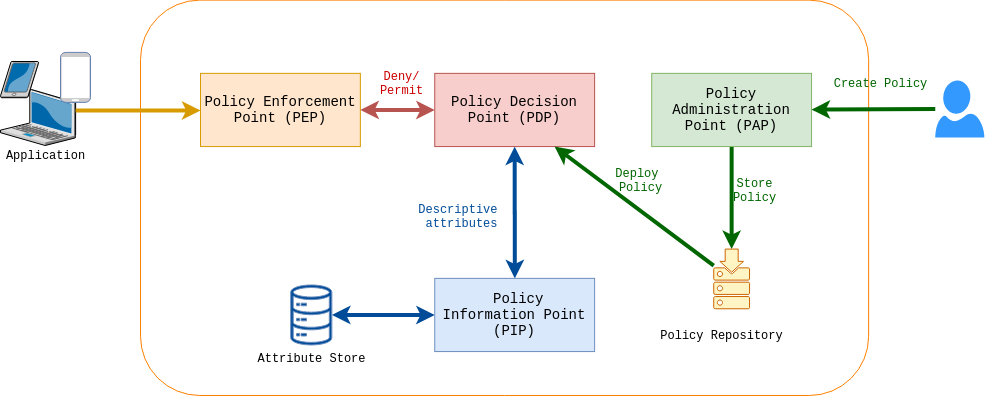
\includegraphics[width=.8\textwidth]{images/XACML.png}
        \caption{XACML Flow-Diagramm}
    
    \end{figure}
    \item \textbf{SAML2}: Hierbei exisitiert ein Identity Provider, an den jeder Service \glqq weiterleitet\grqq{}, um zentral an einer Stelle die Autorisierung zu überprüfen. \cite{Wisniewski.2006}\\
    \begin{figure}[H]
        \centering
        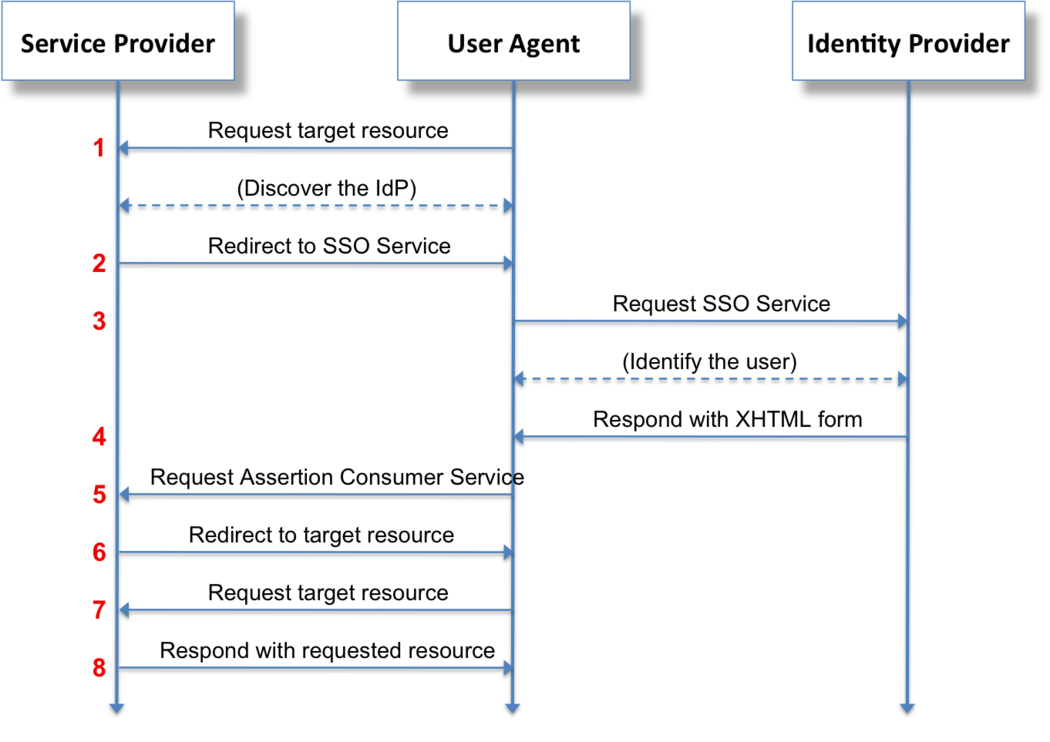
\includegraphics[width=.6\textwidth]{images/SAML.png}
        \caption{SAML Sequenz-Diagramm}
    
    \end{figure}
\end{itemize}

Die detaillierte Beschreibung dieser Standards würde den Rahmen dieser Arbeit übersteigen. Es existieren jedoch viele Ressourcen, um sich diese näher anzusehen.

\paragraph{Verschlüsselung:}
Neben den Diensten selbst, stellen auch die Kommunikationskanäle dazwischen einen Angriffsvektor dar, da diese meist Netzwerkprotokolle verwenden. Um die Integrität, Vertraulichkeit und die Authentizität der Nachrichten zu erfüllen wird der WS-Security (Web-Service Security) Standard verwendet.

WS-Security baut auf SOAP auf und klärt:\begin{itemize}
    \item Wie SOAP-Nachrichten signiert werden um die Integrität sicherzustellen.
    \item Wie SOAP-Nachrichten verschlüsselt werden um Vertraulichkeit zu gewährleisten.
    \item Wie Sicherheitstokens an SOAP-Nachrichten angehängt werden können um die Identität des Absenders sicherzustellen.
\end{itemize}

Die WSS-Spezifikation gibt nicht explizit vor, welche Signaturformate, Verschlüsselungsalgorithmen oder Sicherheits-Token Modelle verwendet werden müssen. Somit kann dieser für die Zukunft geändert werden, falls bessere und neuere Modelle existieren.

Das große Problem bei der Kanalverschlüsselung in SOA ist die große Anzahl der Kanäle. Egal welche Sicherheitsmaßnahmen eingesetzt werden, sie werden immer die Performance beeinträchtigen. 

WSS ist ca. 8 Mal langsamer als herkömmliches HTTPS \cite{Lascelles.2006}, bietet jedoch sichere Funktionalitäten. 

Ein großer Performanceverlust liegt in der Generierung eines neuen Schlüssels für jede geschickte Nachricht. Als Upgrade existiert WSS-Conversation (WSSC), welches gleichzeitige Sessions unterstützt, ohne einen Schlüssel neu definieren zu müssen (verdoppelt den durchschnittlichen Durchsatz) \cite{Lascelles.2006}. 
\section{Auswirkungen auf den Entwicklungsprozess}
\label{ch:developmentProzess}

% Nicht nur Gesamtlösungen entwicklen, sondern generische Komponenten, welche man auf mehreren Systemen entwicklen und einsetzen kann
% isoliert an Systemen entwicklen

% TODO: Was ist der Entwicklungsprozess
% - Wleche Phasen umfasst er

Der Entwicklungsprozess beschreibt den Prozess von der Planung über das Design bis zur letztendlichen Implementierung einer Anwendung. Durch die serviceorientierte Architektur gibt es in einigen Bereichen des Entwicklungsprozesses größere oder kleinere Auswirkungen im Gegensatz zu herkömmlichen Architekturen wie zum Beispiel der monolithischen Architektur. Dabei gibt es bei SOA auch andere Schwerpunkte auf welche bei der Entwicklung zu achten sind. Da es nicht nur einen richtigen Weg gibt, eine SOA zu implementieren können die Schwerpunkte je nach spezifischer Implementierung etwas abweichen. 

Der Software-Entwicklungsprozess hat sich über die letzten Jahrzehnte stark weiterentwickelt. Agile Softwareentwicklung wurde immer populärer und damit einhergehend auch die Entwicklung von verteilten Applikationen. Der serviceorientierte Ansatz für die Softwarearchitektur hat sich dabei zu einer wichtigen Alternative gegenüber der traditionellen Softwareentwicklung entwickelt. \cite{Haines.2010}

\subsection{Feldstudie}
\label{sec:feldstudie}

Um die Veränderungen von SOA auf den Entwicklungsprozess genauer zu untersuchen, wurden im Jahr 2010 in einer Feldstudie Softwareentwickler und IT-Manager aus fünf verschiedenen Unternehmen zu diesem Thema befragt. Bei den gestellten Fragen ging es explizit um die Auswirkungen auf die Softwareentwicklung von SOA basierenden Web-Service. Eines der Unternehmen ist ein Consulting Unternehmen und die restlichen vier Unternehmen sind direkt in der Softwareentwicklung tätig. In jedem der Unternehmen wurde SOA bereits etabliert, oder es war zu dem Zeitpunkt der Umfrage dabei zu SOA umzustellen. Die einzelnen Aussagen der Interviewteilnehmer wurden analysiert, gegeneinander verglichen und zusammengefasst. Zur Validierung der Ergebnisse haben die Teilnehmer im Anschluss noch einmal über die Ergebnisse geschaut. Die Resultate wurden in fünf Phasen des Software-Entwicklungsprozesses eingeteilt. Darunter zählen die Planungsphase, Analysephase, Designphase, Implementierungsphase und die Testphase. \cite{Haines.2010}

Im Folgenden werden die aus der Feldstudie ermittelten Unterschiede von SOA zu herkömmlichen Architekturen, wie zum Beispiel dem Monolithen, erläutert. 


\textbf{Planungsphase}

Die erste Phase ist die Planungsphase. In dieser Phase gibt es größere Veränderungen gegenüber der monolithischen Architektur. Die genaue Umgebung der Applikation ist in einer serviceorientierten Architektur in der Planungsphase noch sehr unbestimmt. Viele Aspekte sind mit SOA deutlich schwerer vorherzusagen und zu kontrollieren, vor allem wenn verschiedene Services von unterschiedlichen Bereichen eines Unternehmens oder sogar von anderen externen Unternehmen stammen. Vor allem in der Planungsphase ist es essenziell, dass effektive Kommunikationskanäle zwischen den verschiedenen Stakeholdern aufgebaut werden. Dies ist zwar auch bei anderen Architekturen nötig, doch für SOA ist es wesentlich wichtiger für einen zukünftigen Projekterfolg. Ein weiterer wichtiger Punkt ist es, Standards festzulegen, welche von den Services eingehalten werden müssen. Darunter fallen zum Beispiel Protokolle zur Kommunikation zwischen verschiedenen Services. An diese Standards muss sich bei der Designphase aller benötigten Services gehalten werden. \cite{Haines.2010}


\textbf{Analysephase}

In der Analysephase fallen die wenigsten Veränderungen im Vergleich zu herkömmlichen Architekturen an. Jedoch ist die Analysephase in SOA ein sehr wichtiger Bestandteil des Entwicklungsprozesses. Ein wichtiger Punkt ist dafür zu sorgen, dass alle verwendeten Datenmodelle und Schemata alle benötigten Daten zur Verfügung haben, da bei SOA im Vergleich zu herkömmlichen Architekturen eine globale Perspektive über alle Services hinweg benötigt wird. \cite{Haines.2010}


\textbf{Designphase}

In der Designphase gibt es wie in der Planungsphase wesentliche Unterschiede im Gegensatz zu herkömmlichen Architekturen. Bei SOA ist es sehr wichtig, dass bei der Designphase von Anfang an alle benötigten Schnittstellen definiert werden. Wenn zu einem späteren Zeitpunkt etwas an den Schnittstellen zwischen den Services geändert werden soll, ist mit einem erheblichen Mehraufwand zu rechnen. Wenn bei herkömmlichen Architekturen mit Schnittstellen gearbeitet wird, ist es ebenfalls wichtig diese schon zu Beginn zu definieren, jedoch sind die Auswirkungen bei Änderungen zu einem späteren Zeitpunkt bei vergleichsweise SOA deutlich verstärkt. Die allgemeine Entwicklung von Schnittstellen verändert sich mit SOA auch stark, da in die Services Standards wie zum Beispiel WSDL eingebunden werden müssen. \cite{Haines.2010}

% TODO: - Was ist WSDL?
%       - Service Granularität
%       - Zu viele externe Services = Schlechtes Design



\textbf{Implementierungsphase}

Auf die Implementierungsphase hat SOA die meisten Auswirkungen. Mit SOA können schnell neue und verbesserte Funktionalitäten implementiert werden, ohne mit anderen Geschäftsprozesse dabei in Konflikte zu geraten. Es ist somit einfacher neue Services bereitzustellen und somit hat SOA eine sehr positive Auswirkung auf die Implementierung. Das Verwalten und Management der einzelnen Services ist nun jedoch ein etwas kritischerer Punkt, da jeder Service ein potenzieller \glqq single point of failure\grqq\ einer Anwendung darstellt. Je nach Aufbau der Anwendung kann man dies zum Beispiel mit redundanten Services beschränken. Bei der Implementierung der einzelnen Services ist in der Implementierungsphase ebenfalls ein hohes Maß an Kommunikation und Koordination zwischen den einzelnen, in den Entwicklungsprozess involvierten Gruppen nötig. Durch unterschiedliche Gruppen besteht jedoch auch die Gefahr, dass Services mehrere unterschiedliche Kanäle zur Kommunikation benötigen. Deswegen ist es wichtig die zuvor spezifizierten Standards für SOA einzuhalten. \cite{Haines.2010}


\textbf{Testphase}

Ebenfalls hat SOA einen großen Einfluss auf die Testphase. Dabei muss vor allem mehr Fokus auf die Integrationstests gelegt werden. Bei den Tests sind zwei verschiedene Umgebungen zu beachten. Eine Umgebung, in welcher die Service-Entwickler möglichst einfach Test-Clients erstellen können, um die Services zu testen und eine weitere Umgebung für Client-Entwickler, welche die entwickelten Applikationen gegen Test-Services testen können. Tools für automatisierte Test-Prozesse spielen dabei ebenfalls eine große Rolle. Nicht nur für funktionale Fehler, sondern auch für die Sicherheit und Performance der Services. Durch die Komplexität der Umgebung sind automatisierte Integration-Tests im Gegensatz zu einer monolithischen Architektur wesentlich wichtiger. \cite{Haines.2010}

\textbf{Ergebnis der Feldstudie}

Die Feldstudie zeigt, dass durch SOA der Entwicklungsprozess teilweise stark angepasst werden muss, um ein effektives Arbeiten zu ermöglichen. Einige Bereiche des Entwicklungsprozesses sind dabei stärker betroffen als andere. Ein größeres Augenmerk muss bei SOA auf die Planungs- und Designphase gelegt werden, um die unterschiedlichen Services inklusive deren Schnittstellen korrekt zu definieren. Die Kommunikation zwischen den verschiedenen Teams hat dabei ebenfalls einen besonders großen Stellenwert. Eine weitere Auffälligkeit ist, dass Änderungen an der anfänglichen Planung mit sehr hohen Kosten bzw. Mehraufwand verbunden sind.


\subsection{Agile Softwareentwicklung}
\label{sec:agileDevelopment}

Agile Softwareentwicklung hat in der Vergangenheit immer mehr an Popularität gewonnen. Damit einhergehend hat der serviceorientierte Ansatz für die Entwicklung immer mehr an Bedeutung gewonnen. Größere Unternehmen können nun mit vielen kleineren Entwicklungsteams unabhängig voneinander parallel an einem Projekt produktiv arbeiten. Somit ist zum Beispiel jedes Team für einen Service zuständig. Bei herkömmlichen monolithischen Ansätzen nimmt die Produktivität ab einer gewissen Teamgröße nicht mehr zu oder sogar ab, da sich die Teammitglieder dabei behindern oder in die Quere kommen. Ebenfalls können in einer Applikation unterschiedliche Programmiersprachen für die Services benutzt werden, und somit auf die Anforderungen des Services oder auf die Kompetenzen des jeweiligen Entwicklungsteams angepasst werden. 

Ein wichtiger Punkt, auf welchen in dem Entwicklungsprozess zu achten ist, ist die Service-Granularität. Die Service-Granularität beschreibt den Funktionsumfang eines einzelnen Services. Bei einer hohen Granularität gibt es somit viele Services mit jeweils sehr kleinem Funktionsumfang und bei einer geringen Granularität gibt es wenige Services mit einem größeren Funktionsumfang.\\
In der agilen Softwareentwicklung geht es um die Reduzierung der Größe und des Umfangs der Probleme, der Reduzierung der Zeit für die Implementierung und die Reduzierung der Zeit um Feedback zu enthalten. Dafür bieten sich eine hohe Service-Granularität und somit kleine Services mit sehr beschränkten Funktionalitäten an. Somit können kleine Services mit einem kleinen Funktionsumfang eigenständig entwickelt werden. Wie klein genau ein Service sein sollte, ist jedoch schwer zu pauschalisieren, geschweige denn zu messen. In der Praxis ist jedoch eine höhere Service-Granularität und somit mehrere auf jeweils einen einzelnen Funktionsbereich zugeschnittene Services vorzuziehen. \cite{NADAREISHVILI.2016}

% Service kann einzeln entwicklet, getestestet und bereitgestellt werden, ohne, dass die gesamte Anwendung neu erstellt werden muss.

\subsection{Modularität und Wartbarkeit}
\label{sec:modularity}

Durch die Services ist ebenso ein höheres Level an Modularität in einer Applikation gegeben. Durch die serviceorientierte Architektur muss nur die Kommunikation unter den Services über die Schnittstellen fest definiert sein. Wie ein Service im inneren aufgebaut ist, ist dabei nebensächlich. Verschiedene Services können somit wiederverwendet werden um redundante Softwareentwicklungen vermeiden. Dabei kann nicht nur der Quelltext wiederverwendet werden, sondern teilweise auch ganze Software-Komponenten. Die entwickelten Service-Komponenten können dabei auch in anderen Anwendungen und Systemen eingesetzt werden, um deren Funktionalität zu erweitern. Durch die Wiederverwendbarkeit der Komponenten kann der Entwicklungsprozess langfristig beschleunigt und die Fehleranfälligkeit reduziert werden. Allerdings gibt es dabei andere Schwerpunkte, worauf geachtet werden muss. Bei größeren Änderungen an Services muss darauf geachtet werden, dass die gesamte Applikation mit allen Services noch funktioniert. Gegebenenfalls müssen dabei noch andere Services angepasst werden. Schwerwiegender wird das Problem, wenn der Service in mehreren Applikationen verwendet wird. Dies ist ein weiterer Grund für die Wichtigkeit der Planungsphase bei einer SOA. 

Neben der Modularität bringt auch die Wartbarkeit aus der Sicht des Entwicklungsprozesses langfristig deutliche Vorteile. Durch die Aufteilung in kleine Services können ohne Beachtung von anderen Services, Updates oder Erweiterungen für einen Service implementiert werden. Späteres Refactoring wird dank simplen Services anstelle einer komplexen monolithischen Applikation ebenfalls deutlich vereinfacht. Bei Funktionsupdates können dabei auch weitere Services ohne Probleme implementiert werden. Bei komplexen monolithischen Applikationen ist bei Funktionsupdates mit einem deutlichen Mehraufwand zu rechnen. Dies trifft vor allem zu, wenn einer Applikation über die Zeit immer weitere Funktionalitäten ohne ein größeres Refactoring hinzugefügt werden oder sich viele Altlasten in dieser befinden. \cite{NADAREISHVILI.2016}

\section{Auswirkungen einer SOA auf den Auslieferungsprozess}
\label{ch:deliveryProcess}
Auslieferung von Software beschreibt den Prozess der Verteilung, Installation beziehungsweise Aktualisierung und Konfiguration von Software für den produktiven Einsatz. Üblicherweise werden hierbei Softwarepakete mit zugehörigen Nutzungsrechten vom Softwarehersteller an den Softwarebetreiber übertragen.\\
Dabei existieren völlig unterschiedliche Herangehensweisen für den Auslieferungsprozess. Je nach Art der auszuliefernden Software und dem späteren Einsatz kann entweder manuell oder automatisiert ausgeliefert werden. Dabei existieren unzählige Zwischenstufen mit unterschiedlichen Automatisierungsgraden. Des Weiteren kann Software beispielsweise entweder über ein Netzwerk oder über ein physisches Installationsmedium ausgeliefert werden. Auch die Art und Frequenz der Durchführung von Aktualisierungen kann sich erheblich unterscheiden. Darüber hinaus existieren viele weitere Möglichkeiten und Eigenschaften, in welchen sich der Auslieferungsprozess eines Softwaresystems unterscheiden kann.\\
Viele der Entscheidungen für die Gestaltung des Auslieferungsprozesses hängen weniger von der Architektur der Software ab als viel mehr von der Art des Systems und von den Wünschen des Kunden. Daher werden viele mögliche Eigenschaften des Auslieferungsprozesses in diesem Abschnitt nicht behandelt. Dennoch ergeben sich aus der Wahl der Softwarearchitektur unterschiedliche Möglichkeiten beziehungsweise Vor- und Nachteile, welche insbesondere bei der Wahl der Verteilungsstrategie ausschlaggebend sind. Einige Verteilungsstrategien werden im nächsten Abschnitt vorgestellt.

Eine wesentliche Eigenschaft von Services ist ihre Eigenständigkeit und Unabhängigkeit. Um diese Eigenschaften auch im Prozess der Auslieferung von serviceorientierten Systemen in größtmöglichem Umfang beibehalten zu können, werden Services üblicherweise in virtuellen Maschinen (VMs) gekapselt und ausgeliefert. VMs sind komplexe Softwaresysteme, die eine isolierte Umgebung auf einem Rechnersystem darstellen. Sie emulieren physische Maschinen und stellen eine Umgebung bereit, welche exakt wie die physische Maschine reagiert, unabhängig von dem tatsächlichen physischen System auf welchem die VM läuft.\\
Der große Vorteil von Virtualisierung ist, dass jegliche Software innerhalb einer VM zunächst vollständig vom außenstehenden System isoliert ist. Zum einen ist ein Service somit von unerwünschtem Zugriff von außen geschützt, da Zugriffsmöglichkeiten zunächst explizit freigegeben werden müssen. Zum anderen ist die Software innerhalb der VM völlig unabhängig von dem physischen System, auf welchem diese läuft, sodass die Software mitsamt der VM auf einen beliebigen anderen virtualisierten Host portiert werden kann. Somit ist ein Service nicht nur positionsunabhängig adressierbar, sondern auch positionsunabhängig ausführbar.\\
Für Microservices werden außerdem oftmals Container für die Kapselung genutzt. Diese haben den Vorteil, dass sie wesentlich leichtgewichtiger sind und somit in sehr dynamischen Systemen eine schnellere Skalierung mit weniger Overhead ermöglichen. Jedoch ist die Software innerhalb eines Containers nicht vollständig isoliert, da beispielsweise mehrere Container auf einem Host denselben Kernel nutzen. Daraus resultieren erhebliche Einbußen hinsichtlich der Sicherheit und Isoliertheit eines serviceorientierten Systems, da sich Software, die in separaten Containern jedoch auf demselben Host läuft, gegenseitig über den Host-Kernel korrumpieren kann.\\
In beiden Fällen wird jedoch eine Kapselung der verwendeten Technologie erreicht, sodass für die Auslieferung und Inbetriebnahme lediglich die API der Virtualisierungs- beziehungsweise Containerisierungslösung bekannt sein muss. Es wird kein weiteres Wissen hinsichtlich der Technologie des Services benötigt. Die Vorteile im Auslieferungsprozess werden allerdings mit erhöhter Komplexität beim Bauprozess aufgewogen, da hier zusätzlich die Images für die VMs oder Container erstellt werden müssen.\\
Die Verwendung einer SOA und die gewonnene Flexibilität durch die daraus resultierende lose Kopplung ermöglicht zusätzlich eine wesentlich agilere Auslieferung von Aktualisierungen und flexiblere Möglichkeiten für die Skalierung eines Softwaresystems.\\
Im Folgenden werden diese Möglichkeiten genauer erläutert.

\subsection{Skalierung}
\label{sec:scaling}
Ein System, bestehend aus autonomen Services kann sowohl horizontal als auch vertikal unproportional skaliert werden. Unproportionale Skalierung meint hierbei, dass einzelne Services des Systems in beliebige Richtung skaliert werden können, während andere Services ihre Kapazität halten. Somit kann sich das Gesamtsystem dynamisch an beliebige Lastszenarien anpassen \cite{NADAREISHVILI.2016}.\\
Weitere oder leistungsfähigere Serviceinstanzen können somit bei Bedarf ausgeliefert und zugeschaltet werden. Man nennt dieses Vorgehen auch \textit{deploy on demand}.\\
Dabei sollte beachtet werden, dass eine Skalierung lediglich dann erfolgen sollte, wenn mittel- oder langfristige Lastveränderungen im System auftreten oder eine Lastveränderung aufgrund eines vorhersehbaren Ereignisses bevorsteht. Die ständige Anpassung an kurzfristige Szenarien sorgt ansonsten für enormen Overhead aufgrund der Auslieferung und Inbetriebnahme beziehungsweise dem Herunterfahren von Services. Zusätzlich erfolgen ständige Änderungen im Lastenverteilungssystem durch zu- beziehungsweise abschalten neuer Services oder Ressourcen.\\
Vertikale Skalierung beschreibt in diesem Kontext die Erhöhung beziehungsweise Reduktion der verfügbaren Ressourcen eines Services. Dies kann beispielsweise bedeuten, eine Serviceinstanz durch eine andere zu ersetzen, die auf einem leistungsfähigeren Host läuft oder die zugeteilten Ressourcen der VM, in welcher die Serviceinstanz läuft, zu erhöhen \cite{NADAREISHVILI.2016}.\\
Bei der horizontalen Skalierung werden mehrere Instanzen des gleichen Services eingerichtet und zugeschaltet. Die Gesamtlast des Systems wird dann über ein Lastenverteilungssystem auf die unterschiedlichen Instanzen aufgeteilt.\\
Abbildung \ref{fig:scaling} stellt die unterschiedlichen Skalierungsmöglichkeiten bildlich dar.

\begin{figure}[H]
    \centering
    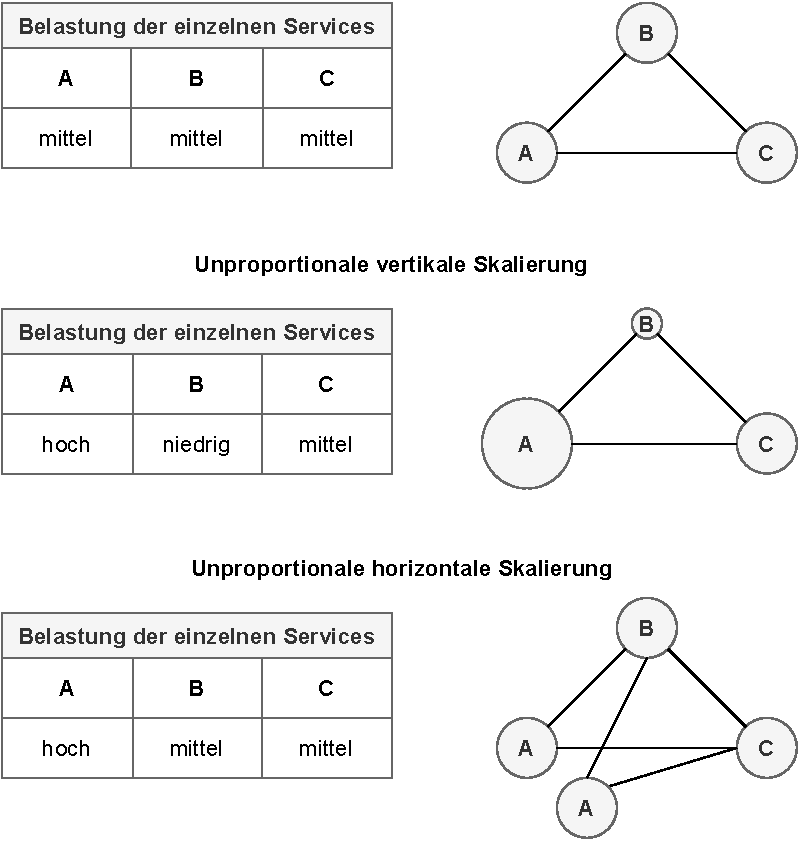
\includegraphics[width=0.8\textwidth]{images/scaling.pdf}
    \caption{Darstellung der beispielhaften Skalierungsmöglichkeiten eines Systems bestehend aus drei Services A, B und C, entsprechend bestimmter Lastszenarien}
    \label{fig:scaling}
  \end{figure}

\subsection{Aktualisierung}
\label{sec:update}
Wie bereits im Zusammenhang mit dem Entwicklungsprozess erläutert, bietet die lose Kopplung viele Möglichkeiten für die agile Weiterentwicklung eines serviceorientierten Systems. Einzelne Services können beispielsweise vollständig unabhängig voneinander weiterentwickelt und aktualisiert werden.\\
Daraus resultieren zumeist wesentlich frequentiertere Rollouts. Änderungen können auf Serviceebene ausgeliefert werden. Somit kann das Gesamtsystem kleinschrittig weiterentwickelt und aktualisiert werden, ohne dass jemals das komplette System neu aufgesetzt werden muss. Dabei ist zu beachten, dass dies nur möglich ist, wenn die Schnittstellen der einzelnen Services lediglich erweitert, nicht aber verändert oder verkleinert werden. Ansonsten kann es zu Inkompatibilitäten innerhalb des Gesamtsystems kommen. 

Im Folgenden werden nun drei Verteilungsstrategien für die Auslieferung von Aktualisierungen eines SOA Systems vorgestellt \cite{STORZ.2021}.

\textbf{Rollende Auslieferung}

Bei der rollenden Auslieferung von Services werden in einer geklusterten Umgebung nach und nach einzelne Hosts aus der Produktivumgebung genommen. Die neue Version wird auf dem Host eingerichtet. Anschließend wird der Host wieder in die Produktivumgebung eingepflegt. Dies ermöglicht die schrittweise Aktualisierung des gesamten Systems.\\
Der Vorteil ist, dass nicht direkt alle Instanzen aktualisiert werden, wodurch das Risiko im Fehlerfall begrenzt wird. Außerdem ist die Umsetzung der rollenden Auslieferung relativ einfach. Nachteil an dieser Verteilungsstrategie ist, dass einzelne Hosts zeitweise vom Netz genommen werden.\\
Abbildung \ref{fig:rolling} visualisiert den Ablauf einer rollenden Aktualisierung.\\

\begin{figure}[H]
  \centering
  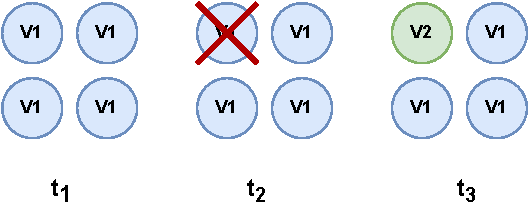
\includegraphics[width=0.5\textwidth]{images/rolling.pdf}
  \caption{Ablauf einer rollenden Aktualisierung}
  \label{fig:rolling}
\end{figure}

\textbf{Blue-Green Auslieferung}

Es wird parallel eine zweite Server-Instanz mit dem aktualisierten Service gestartet. Anschließend werden alle Nachrichten, die an den Service adressiert sind, über ein Lastenverteilungssystem an die aktualisierte Instanz geleitet. Im Falle eines Fehlers wird die Last wieder auf die alte Instanz geleitet. Tritt kein Fehler auf, so kann die alte Instanz heruntergefahren werden.\\
Vorteil dieser Strategie ist, dass praktisch keine Downtime auftritt. Außerdem kann ein Rollback relativ einfach realisiert werden, indem die Last wieder auf die alte Instanz geleitet und die aktualisierte Instanz wieder heruntergefahren wird.\\
Der Nachteil dieser Strategie ist, dass im Falle eines Fehlers 100 \% der Benutzer betroffen sind, bis der Fehler erkannt und die Last wieder auf die alte Instanz umgeleitet ist.\\
Abbildung \ref{fig:blue-green} visualisiert den Ablauf einer Blue-Green Aktualisierung.\\

\begin{figure}[H]
  \centering
  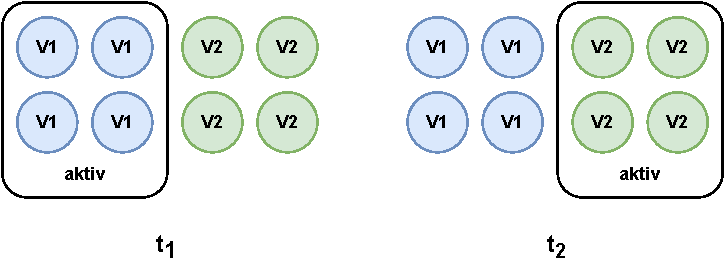
\includegraphics[width=0.7\textwidth]{images/blue-green.pdf}
  \caption{Ablauf einer Blue-Green Aktualisierung}
  \label{fig:blue-green}
\end{figure}

\textbf{Canary Auslieferung}

Die Canary Strategie ähnelt der Blue-Green Strategie, soll jedoch deren Probleme bei Auftreten eines Fehlers beheben. Sie kann angewendet werden, wenn jeweils mehrere Instanzen der zu aktualisierenden Services im System aktiv sind. Bei der Canary Strategie werden zunächst nur wenige aktualisierte Serviceinstanzen gestartet. Ein Teil der Anfragen werden anschließend über das Lastenverteilungssystem auf die neuen Instanzen geleitet. Treten bei der Benutzung keine Fehler auf, werden anschließend alle zu aktualisierenden Services im Blue-Green Verfahren ersetzt. Die Verwendung der Canary Strategie ist nur möglich, wenn gleichzeitig mehrere Versionen eines Services laufen können.\\
Vorteil dieser Strategie ist, dass im Fehlerfall nur eine Teilmenge der Benutzer betroffen ist. Außerdem gelten die gleichen Vorteile, die bereits bei der Blue-Green Strategie genannt wurden.\\
Der Nachteil dieser Strategie ist eindeutig die Komplexität in der Umsetzung. Die Verwendung der Canary Strategie ist nur zu empfehlen, wenn sie über ein Continuous Delivery (CD) System automatisiert ist.\\
Abbildung \ref{fig:canary} visualisiert den Ablauf einer Canary Aktualisierung.\\

\begin{figure}[H]
  \centering
  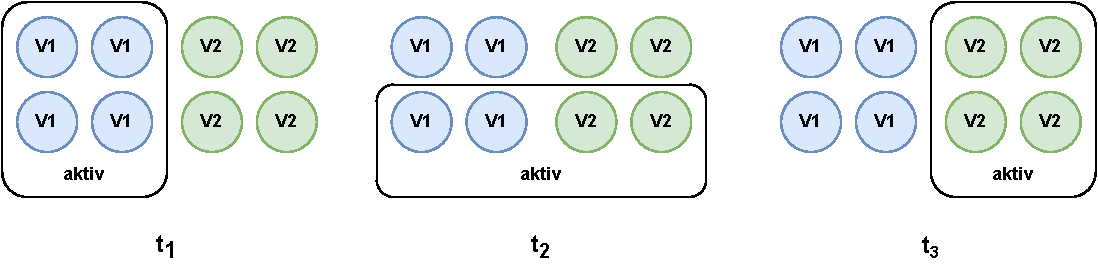
\includegraphics[width=\textwidth]{images/canary.pdf}
  \caption{Ablauf einer Canary Aktualisierung}
  \label{fig:canary}
\end{figure}


\subsection{Zusammenfassung der Auswirkungen}
\label{sec:deploymentSummary}
Es wurden unterschiedliche Aspekte der Auslieferung von serviceorientierten Systemen beleuchtet. Im Folgenden werden nun die konkreten Auswirkungen einer SOA auf den Auslieferungsprozess von Softwaresystemen zusammengefasst.

Zunächst ist die Einrichtung der einzelnen Services, unabhängig der Implementierungs-Technologie über das API der Virtualisierungs- oder Containersoftware ein wichtiger Punkt.\\
Virtualisierung wird zwar auch bei Systemen mit anderen Architekturen verwendet, ist aber zentral für SOA, da sie homogene Auslieferungs- und Installationsprozesse für heterogene Services ermöglicht.

Auch die verteilte Auslieferung der Systeme und die daraus resultierende erhöhte Komplexität des Auslieferungsprozesses ist eine zentrale Auswirkung der Verwendung einer SOA.\\
Alle Services des Systems müssen einzeln ausgeliefert werden und werden zudem üblicherweise auf unterschiedlichen Hosts eingerichtet. Dadurch wird der Auslieferungsprozess wesentlich komplexer als beispielsweise die Auslieferung eines monolithischen Systems.\\
Um diese Komplexität zu verringern, wird zunehmend \textit{serverlos} ausgeliefert. Dabei wird der Code der Services an einen Anbieter für serverlose Auslieferung weitergegeben, welcher dann beliebig viele Instanzen in gewünschter Konfiguration auf eigener Infrastruktur ausliefert. Dabei übernimmt dieser Anbieter die gesamte Verwaltung der Infrastruktur und stellt die Funktionalität der Services über ein Netzwerk bereit. Die Verwendung einer serverlosen Auslieferung hat den Vorteil, dass der Auslieferungsprozess erheblich vereinfacht wird und keine eigenen Hosts mehr verwaltet werden müssen. Im Austausch mit diesen Vorteilen stehen die Vertrauenswürdigkeit der Anbieter und die Tatsache, dass der Herausgeber der Services keinerlei Kontrolle darüber hat, wo diese laufen \cite{STORZ.2021}.

Auch die Auswirkungen auf die Skalierung eines Systems wurden bereits beschrieben. Bei der Auslieferung von monolithischen Systemen wird beispielsweise eine Instanz des Systems auf einem Host eingerichtet. Um diese Systeme skalieren zu können, wird je nach Art des Systems entweder die bestehende Instanz auf einen leistungsfähigeren Host verschoben oder es werden weitere Instanzen des Systems auf anderen Hosts aufgesetzt, die sich die vorhandene Last anschließend teilen.\\
Bei serviceorientierten Systemen werden die einzelnen Services hingegen einzeln ausgeliefert und skaliert.\\
Für die flexible Skalierbarkeit der Systeme und dem damit einhergehenden \textit{deployment on demand} wird eine Art Service Provider benötigt, der bei Bedarf weitere oder leistungsfähigere Serviceinstanzen bereitstellen und ausliefern kann \cite{NADAREISHVILI.2016}. Diese Möglichkeiten führen zu deutlich erhöhter Komplexität der Infrastruktur, wenngleich sie enorme Vorteile für die Flexibilität eines Systems bieten.

Eine weitere Auswirkung der SOA auf den Auslieferungsprozess sind wesentlich kleinschrittigere Aktualisierungen und daraus resultierend wesentlich frequentiertere Auslieferungen ohne Downtime des Systems (beispielsweise durch Blue-Green oder Canary Auslieferung).

Insgesamt ist also erkennbar, dass die Verwendung einer SOA zu einem komplexeren Auslieferungsprozess führt. Um diese Komplexität handhabbar zu machen, werden zumeist umfangreiche DevOps Systeme für die Unterstützung im Entwicklungs- und Auslieferungsprozess verwendet.\\
Diese führen bei zielgerichteter Benutzung zu einer besseren Organisation, die sich bereits im Entwicklungsprozess positiv auswirkt. So ist beispielsweise eine gut organisierte Quellcodeverwaltung eine essenzielle Basis, um die isolierte Entwicklung homogener Services gut strukturiert durchführen zu können und aus diesen zu einem späteren Zeitpunkt komplexe Systeme zusammensetzen zu können. Darüber hinaus unterstützen diese Systeme das Konfigurations- und Releasemanagement, um die Zusammensetzung, Parametrisierung und Versionierung der serviceorientierten Softwarelösungen zu automatisieren. Dies reduziert Fehler und Inkonsistenzen, sowohl im Stadium der Entwicklung, als auch im Auslieferungsprozess. Eine gute Organisation und konsistente Daten sind beispielsweise auch nötig, um Systeme für Wartungsarbeiten, Recovery- und Testszenarien reproduzierbar zu machen.\\
In vielen DevOps Systemen lassen sich außerdem sogenannte \textit{Pipelines} einrichten, über welche umfangreiche Ausführungsfolgen automatisiert werden können. Eine solche Pipeline kann zum Beispiel nach Fertigstellung einer Aktualisierung automatisiert gestartet werden. Im Durchlauf der Pipeline werden dann beispielsweise die Paketierung und Einrichtung der Software in einer VM angestoßen werden und der aktualisierten Service wird als VM-Image für den Kunden bereitgestellt oder direkt auf dessen Zielhosts ausgerollt.

Die Möglichkeit, Systeme in Form von einzelnen Services auszuliefern und dadurch unabhängig voneinander erweitern, skalieren und aktualisieren zu können, birgt je nach Anwendungsfall also enorme Vorteile, führt im gleichen Zug jedoch auch zu erheblicher Steigerung der Komplexität bei der Auslieferung. Diese Komplexität kann durch geeignete Hilfssysteme zwar wieder reduziert werden, dies ist jedoch mit sehr hohem initialen Aufwand verbunden.\\
Die Verwendung einer SOA lohnt sich hinsichtlich der Auswirkungen auf den Auslieferungsprozess also nur, wenn die dadurch gewonnenen Vorteile auch ausgeschöpft werden.
\newpage
\pagenumbering{Roman}
\setcounter{section}{0}
\setcounter{secnumdepth}{0}

\newpage
%%% Angabe der .bib-Datei (ohne Endung) / State .bib file (for BibTeX usage)
\printbibliography%\printbibliography if you use biblatex/Biber
\end{document}